\begin{frame}
\frametitle{Functions of Several Variables}

\begin{itemize}
\item Verbal description

\item Numerical description

\item Analytical description

\item Graphical description

\end{itemize}
\end{frame}

\begin{frame}
\frametitle{Verbal Description}

\begin{itemize}
\item The wind chill temperature: apparent temperature felt on exposed skin.

Depends on:
\begin{itemize}
\item the actual temperature, $T$;
\item the wind speed, $v$;
\item the humidity.
\end{itemize}

Assumption: zero humidity.
 %
  $$W = W(T,v)\; .$$
  %

  \item Rectangular coordinates of a point with given spherical coordinates:
  %
  $$(x,y,z) = \textbf{F}(\rho, \theta, \phi)\; ,$$
  %

  \item The electric force on a charge $q$ displaced
  by $\textbf{r}$ from a charge $Q$
  
  Depends on:
  \begin{itemize}
  \item the two charges, $q$ and $Q$;
  \item the displacement $\textbf{r}$;
  \item  the medium in which the charges are placed
  \end{itemize}
  %
  $$\textbf{E} =
  \textbf{E}(q, Q,\textbf{r}, \varepsilon)\; .$$
  %
 

\end{itemize}
\end{frame}

\begin{frame}
\frametitle{Numerical Description}

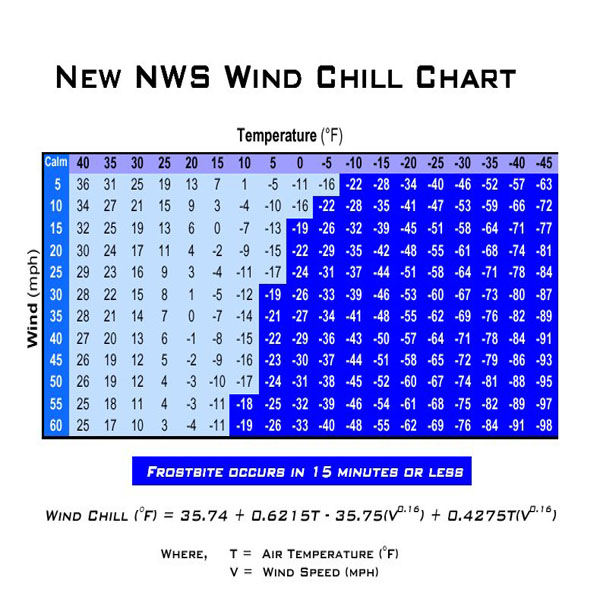
\includegraphics[width=3in]{../images/windchill2.jpg}
\end{frame}

\begin{frame}
\frametitle{Analytical Description}

\begin{itemize}
  \item Windchill temperature:
  %
  $$W(T,v)= 35.74+0.6215 T - 35.75 v^{0.16} +0.4275 Tv^{0.16}$$
  %
  with $W$ and $T$ in Fahrenheit and $v$ in $mph$.

 \item The transition formulas from spherical to
    rectangular coordinates.
$$
\begin{cases}
x &= \rho \sin\phi \cos\theta \\
%
y &= \rho \sin\phi \sin\theta \\
%
z &= \rho \cos\phi
\end{cases}
$$

  \item The Cobb-Douglas production function:
   %
  $$P(K,L) = cL^a K^{1-a}\; ;$$
    %


    \item Coulomb's Law: 
        %
    $$\textbf{E}(q, Q, \textbf{r}, \varepsilon) =
    \frac{\varepsilon q Q}{|\textbf{r}|^3} \textbf{r}\; ,$$
    %
 
\end{itemize}

\end{frame}

\begin{frame}
\frametitle{Graphical Descriptions: Graphs}
%
$$(T, v, W(T,v)) \longrightarrow z=f(x,y)$$
%
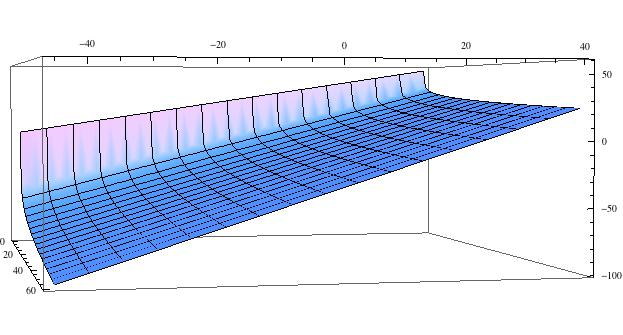
\includegraphics[width=4in]{../images/windchill-graph.jpg}
\end{frame}

\begin{frame}
\frametitle{Graphical Description: Contour lines}
%
$$W(T,v) = c \longrightarrow f(x,y) = c$$
%
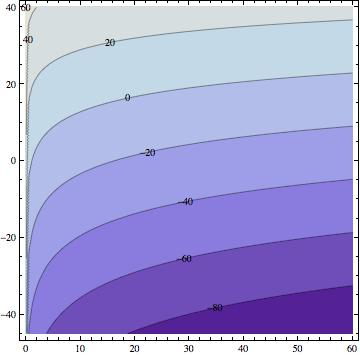
\includegraphics[width=2in]{../images/windchill-contour.jpg}
\end{frame}
